\subsection{Results}

\subsubsection{Jittering}

\subsubsection{Clipping}
A set of infinite clipping planes can be defined to clip the volume to reveal inner detail, as shown in Figure 4.  Clipping is implemented by determining the visibility of each sample along the ray according to whether that location is excluded by the clipping planes.A set of infinite clipping planes can be defined to clip the volume to reveal inner detail, as shown in Figure 4.  Clipping is implemented by determining the visibility of each sample along the ray according to whether that location is excluded by the clipping planes.

\subsubsection{Cropping}
Cropping refers to 27 regions that defined by two planes along each coordinate axis of the volume and can be independently turned on (visible) or off (invisible) to produce a variety of different cropping effects, as shown in Figure~\ref{fig:cropping}. Cropping is implemented by determining the cropping region of each sample location along the ray and including only those samples that fall within a visible region.

\begin{figure}
\centering
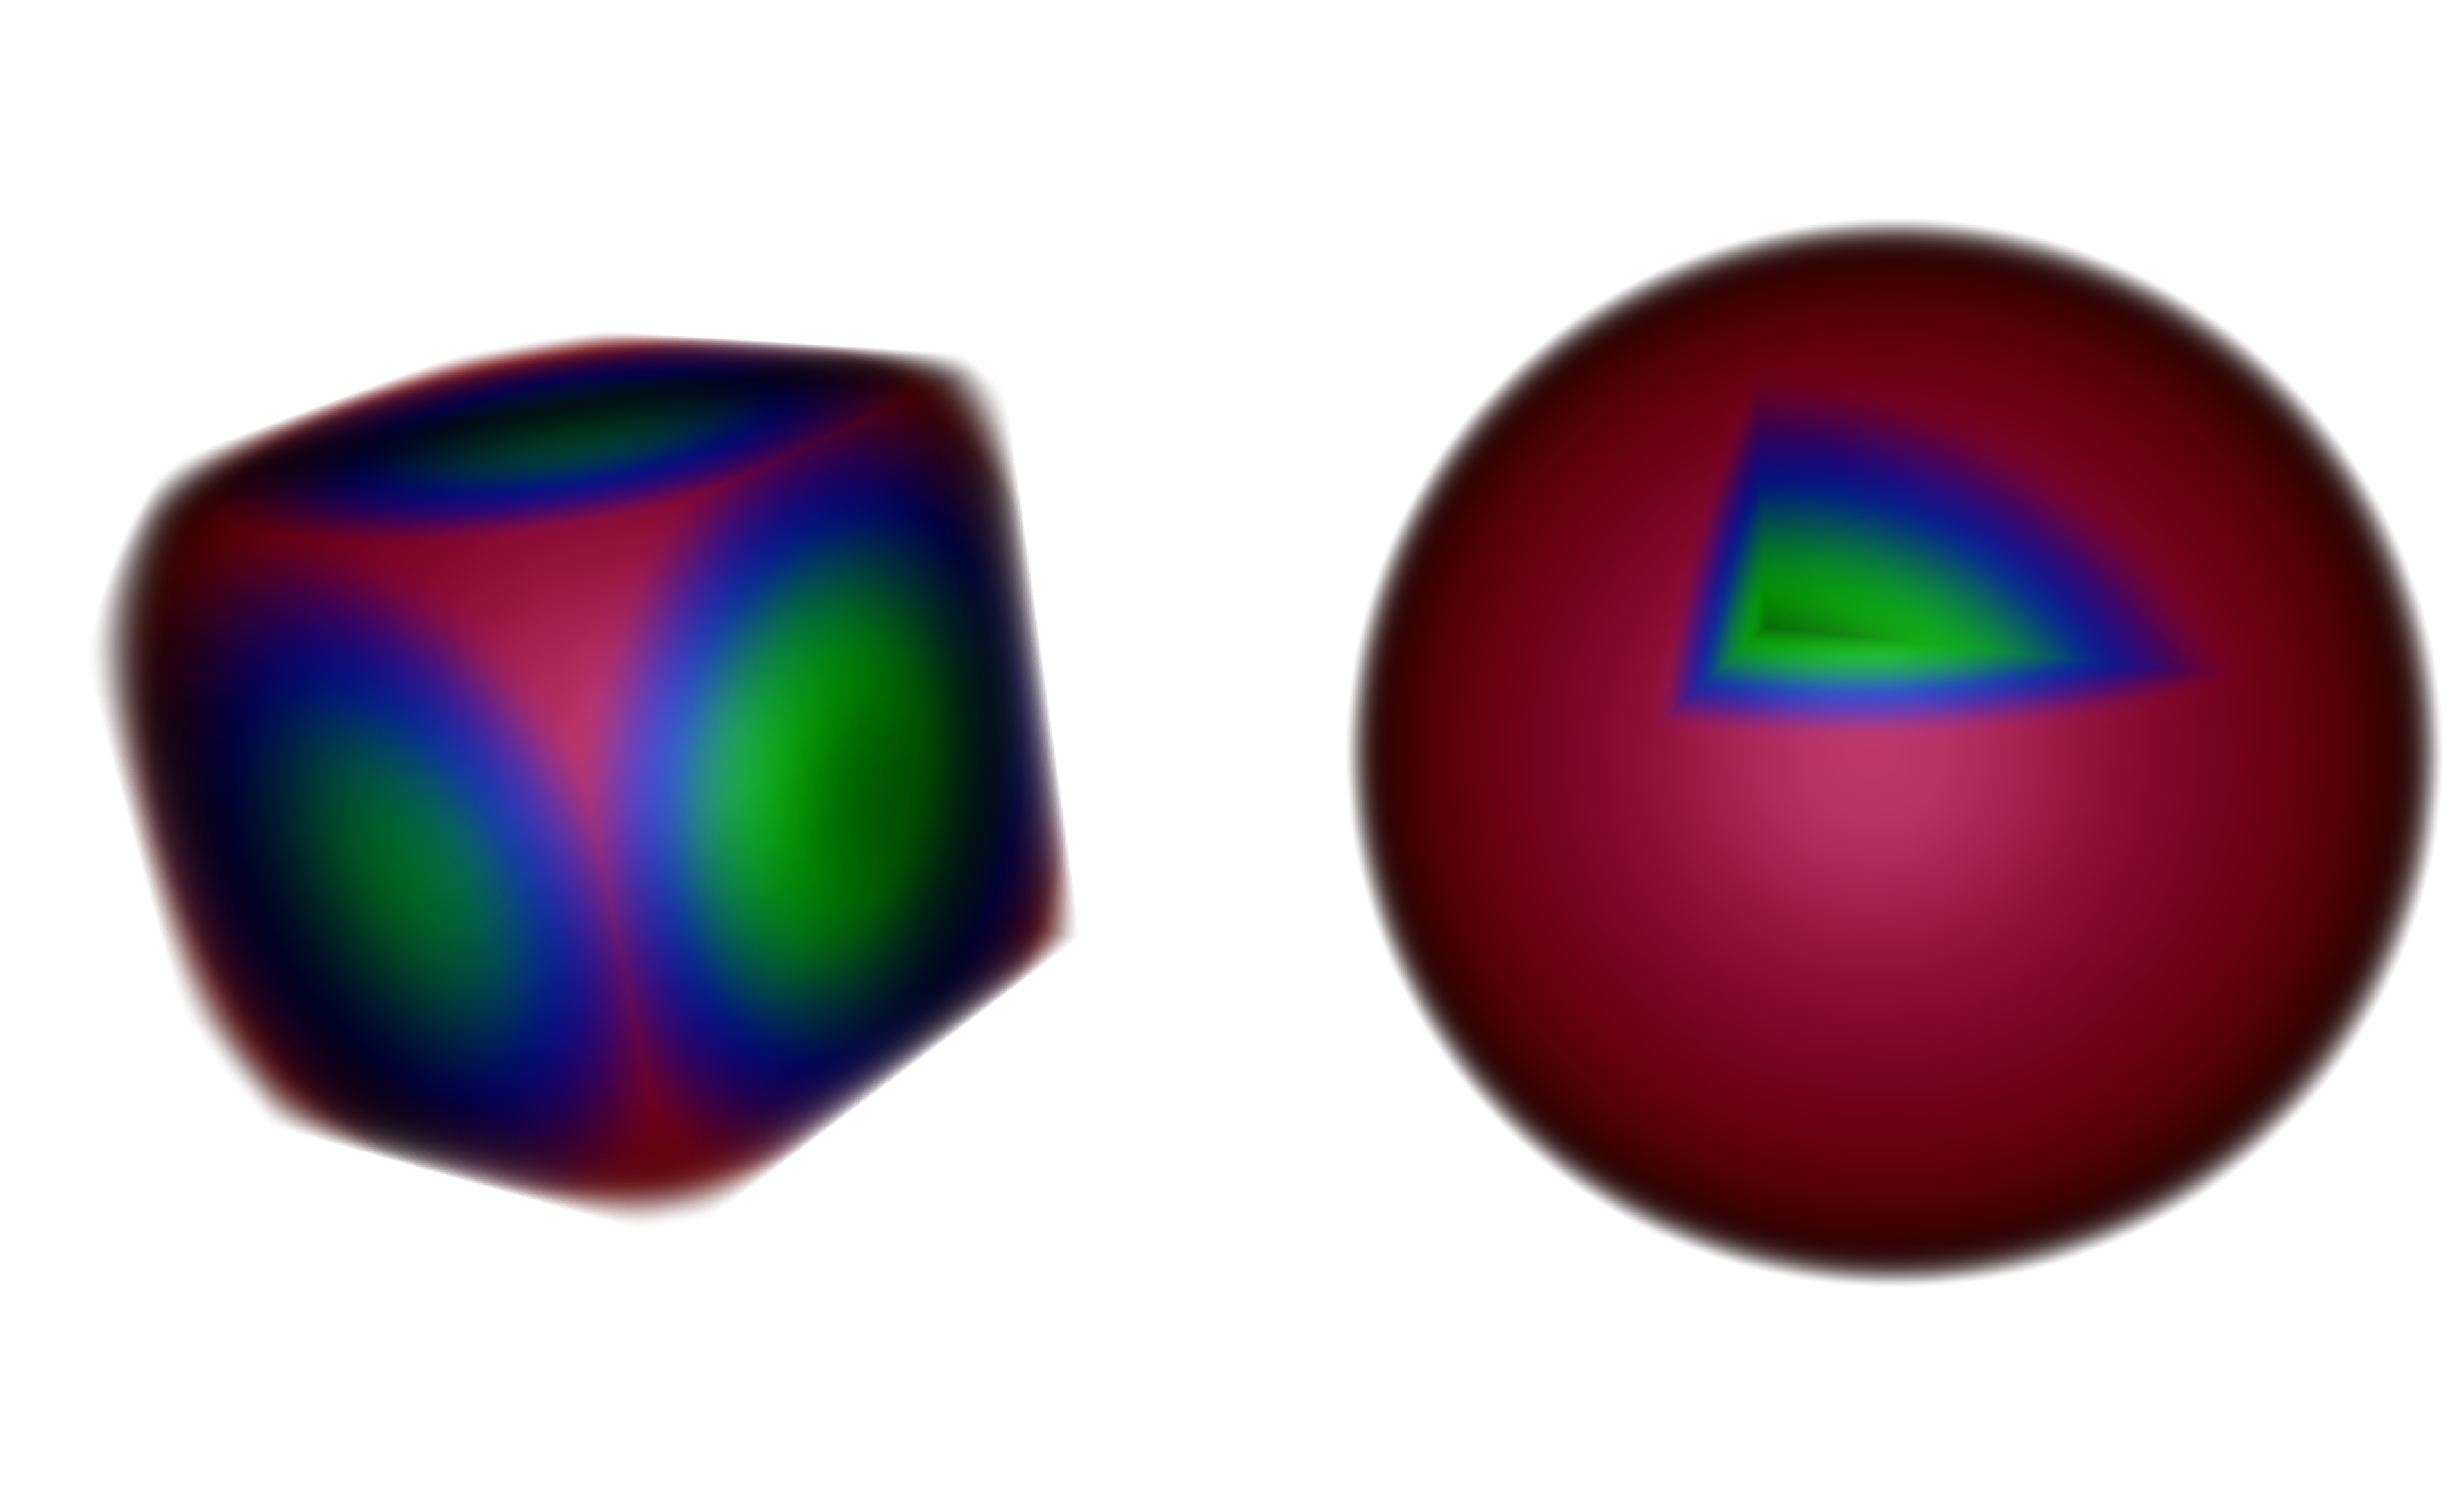
\includegraphics[width=2.5in]{SphereCropping.png}
\caption{Figure 3. A sphere is cropped using two different configurations of cropping regions.}
\label{fig:cropping}
\end{figure}

\subsubsection{Wide Support of Data Types} 
The vtkGPURayCastMapper supports most data types such as short, int, float, and double and both point and cell data types. Bias are scale are computed and applied to the scalars in the fragment shader to normalize the scalars between 0-1 range. 

\begin{figure}
\centering
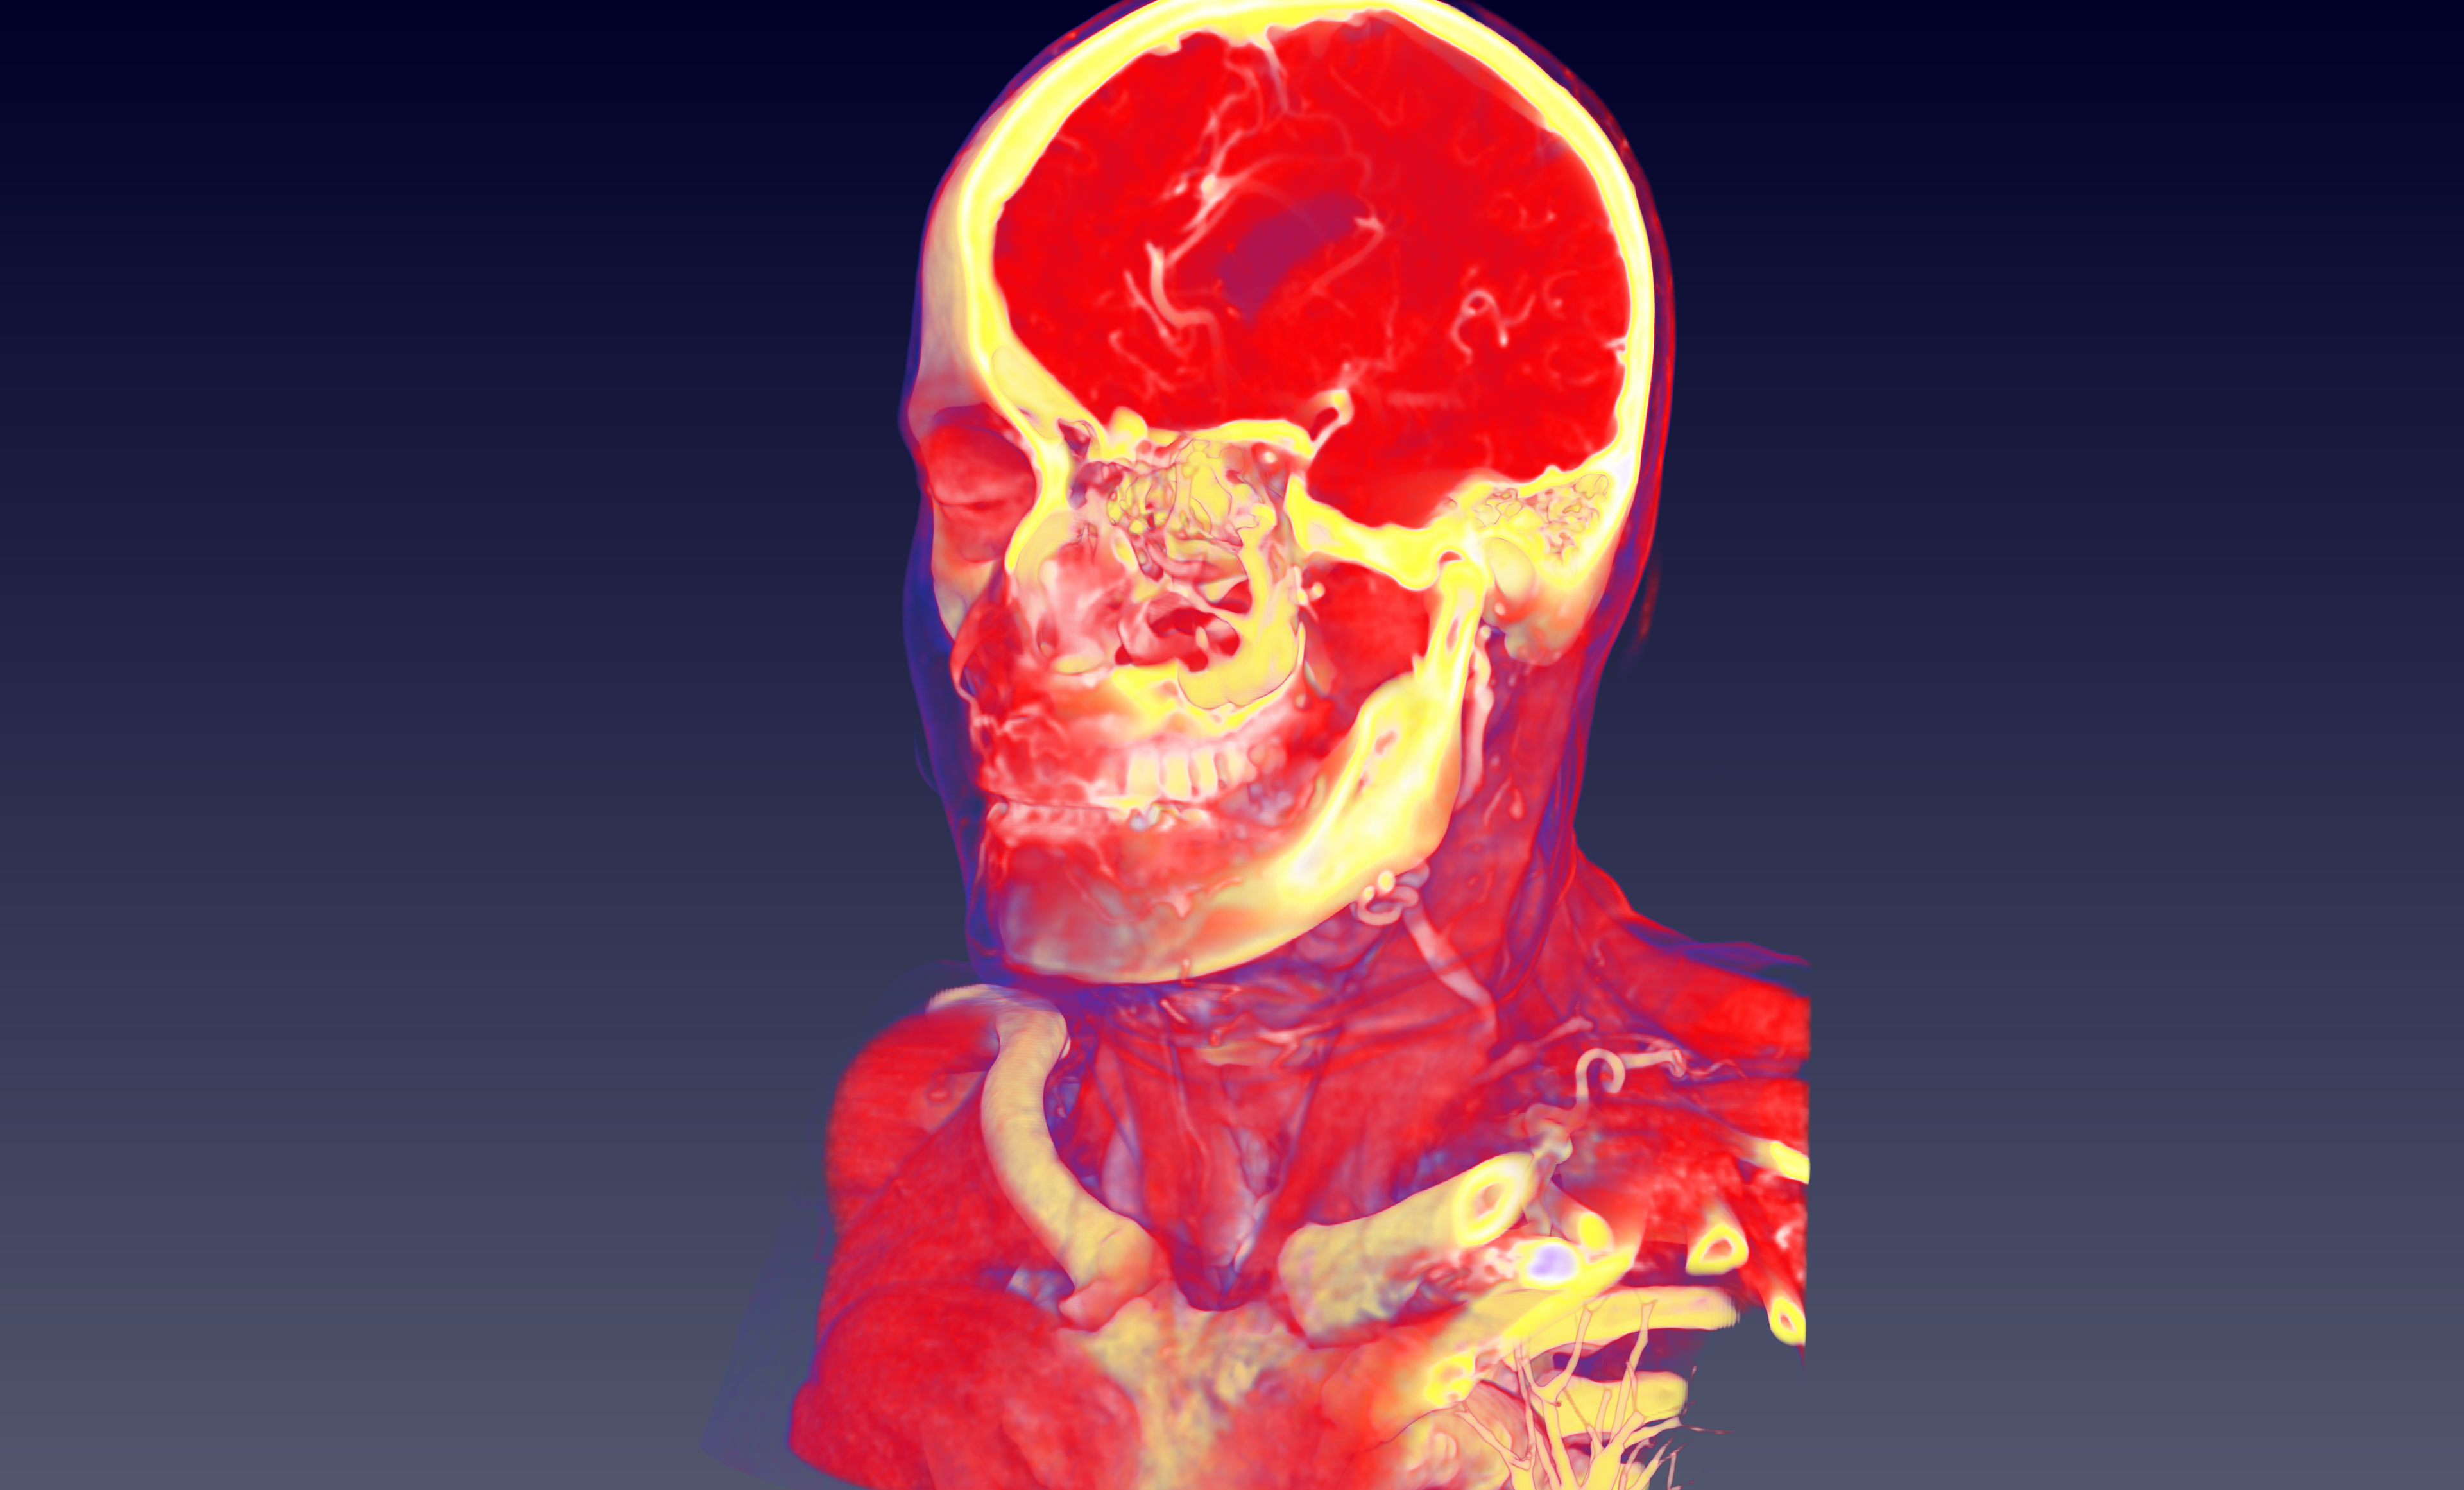
\includegraphics[width=2.5in]{HeadClippingOblique.png}
\caption{Figure 4. Top: An example of an oblique clipping plane. Bottom: A pair of parallel clipping planes clip the volume, rendered without (left) and with (right) shading.}
\label{fig:clipping}
\end{figure}

\subsubsection{Blending Modes *Sankhesh to add new blending mode}
The mapper supports composite blending, minimum intensity projection, maximum intensity projection, and additive blending. Each of these blending modes are useful for a particular use-case in medical computing. The most common one which is also the default is the composite blending mode. See Figure~\ref{fig:blendingmodes} for an example of composite blending, maximum intensity projection, and additive blending on the same data.

\begin{figure*}
\centering
\begin{subfigure}{.6\columnwidth}
    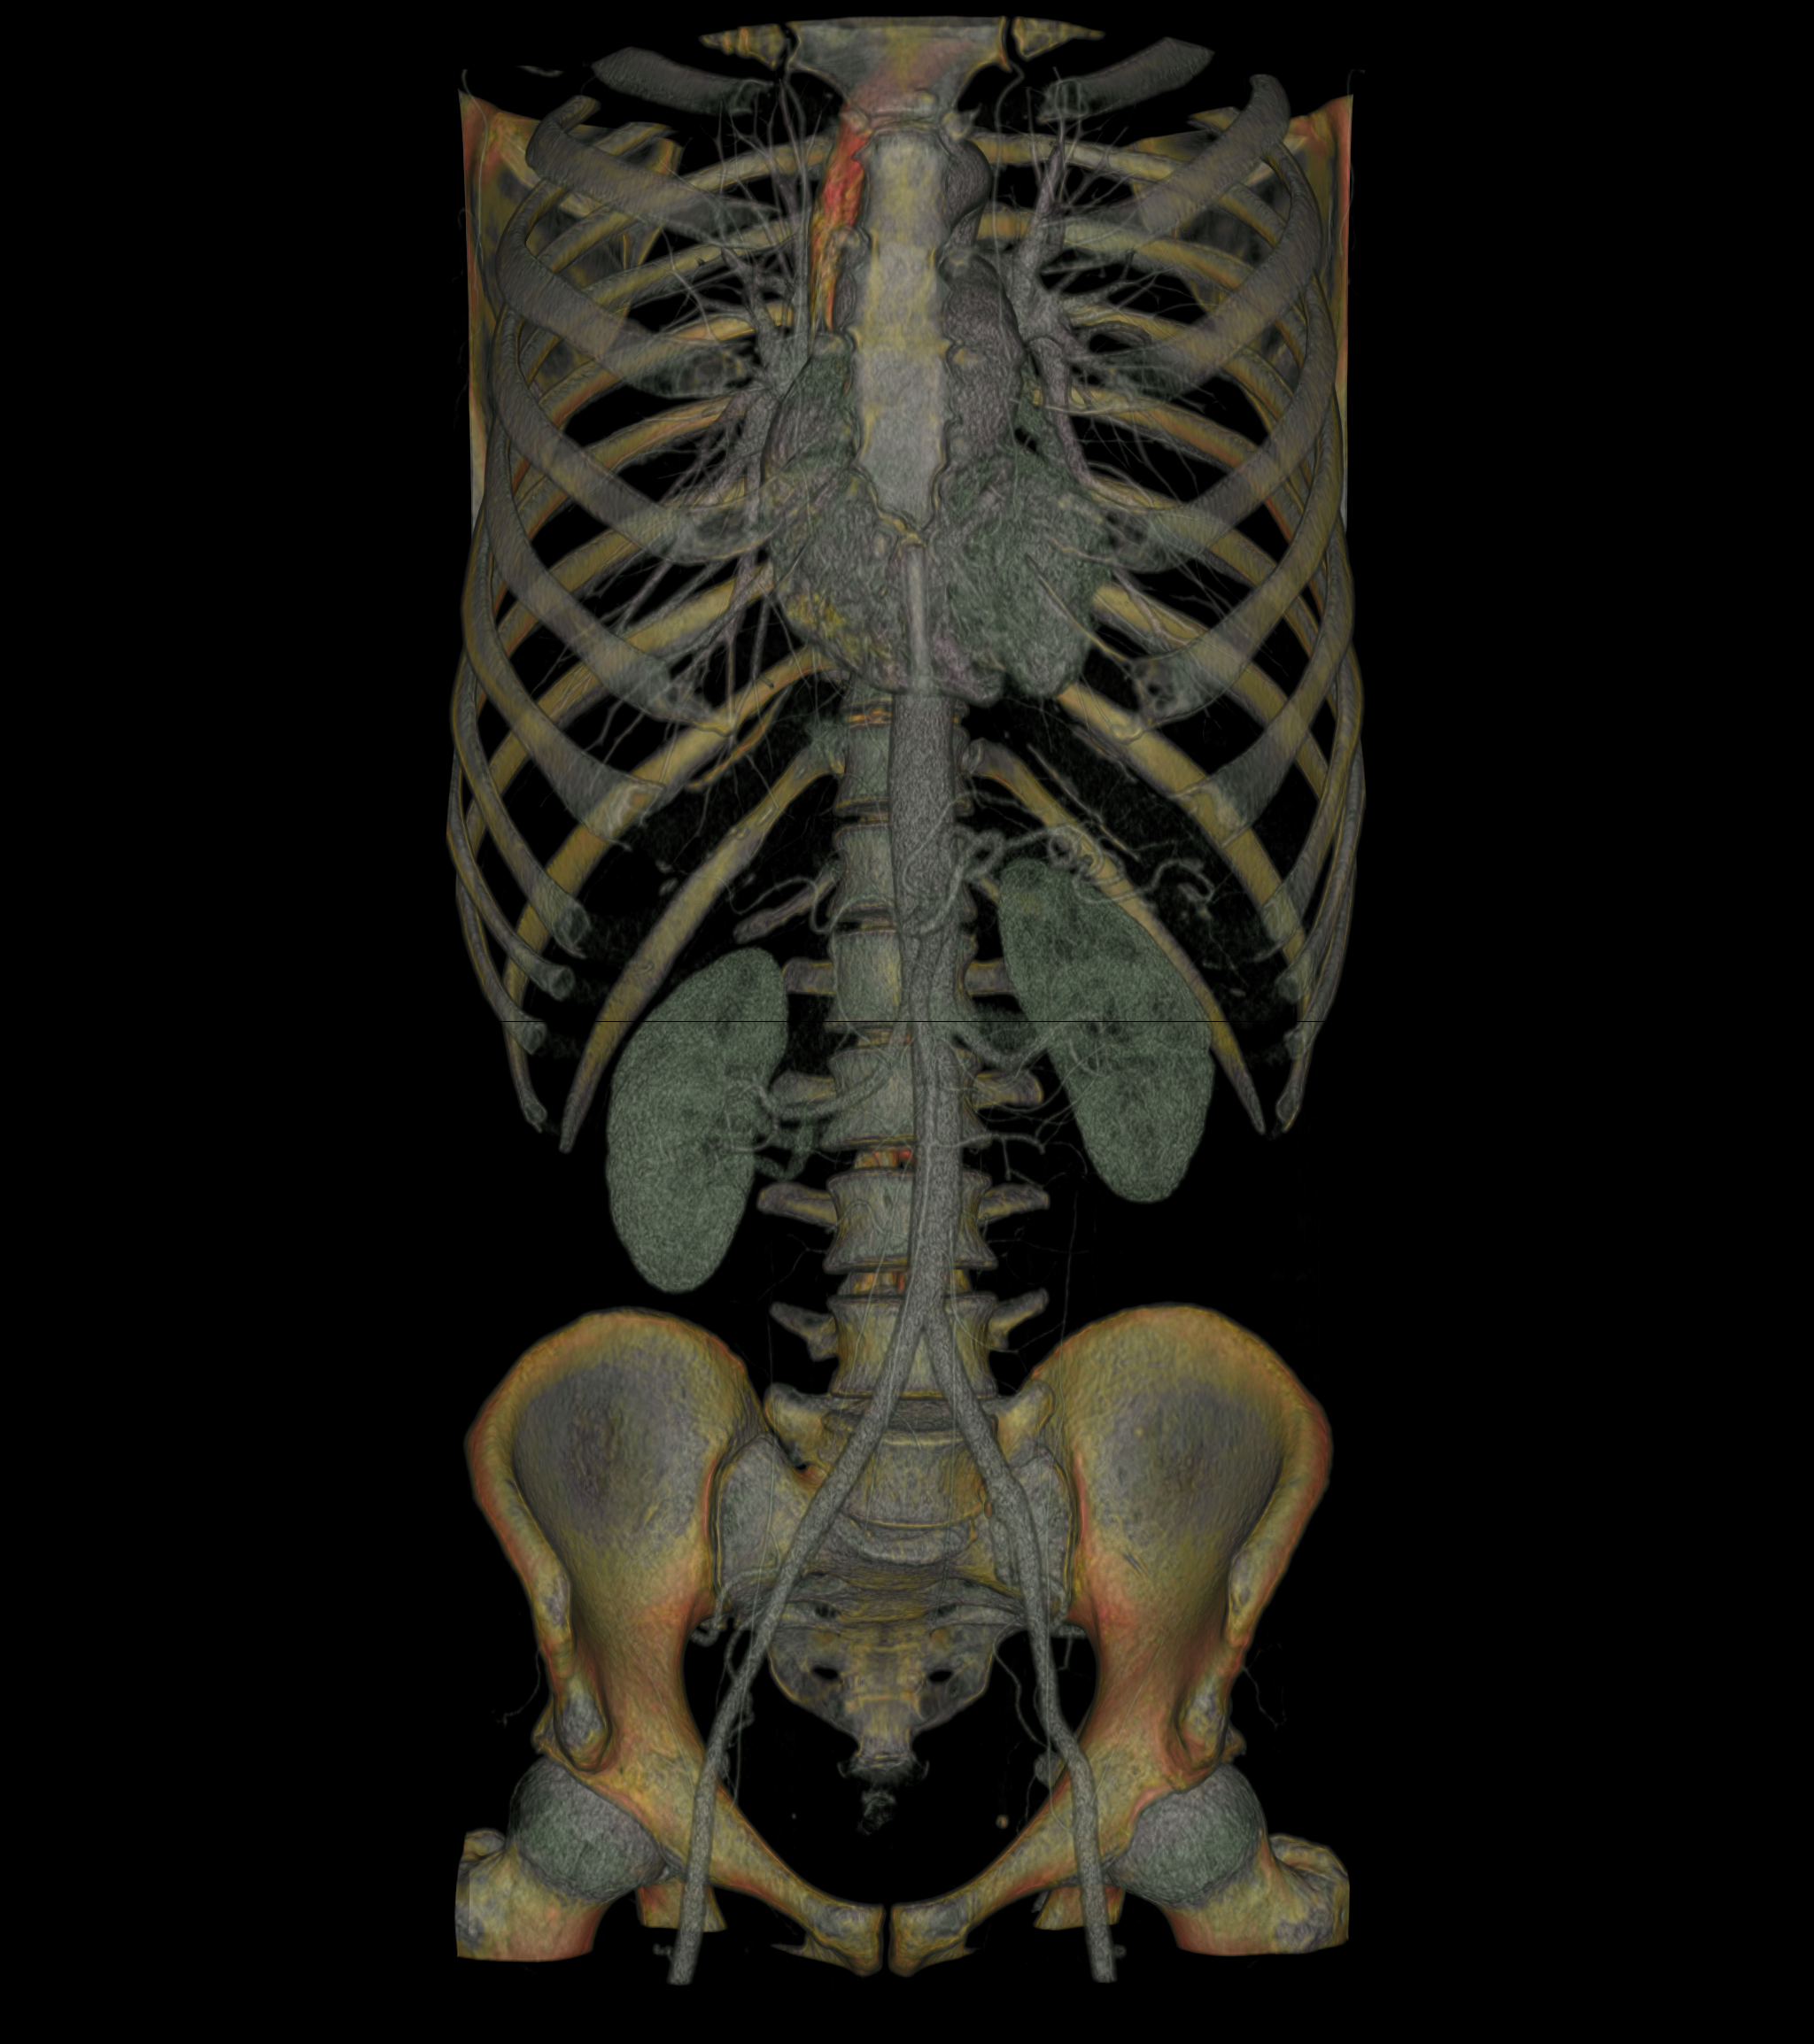
\includegraphics[width=\columnwidth]{TorsoBlendingComposite.png}
\end{subfigure}
\begin{subfigure}{.6\columnwidth}   
    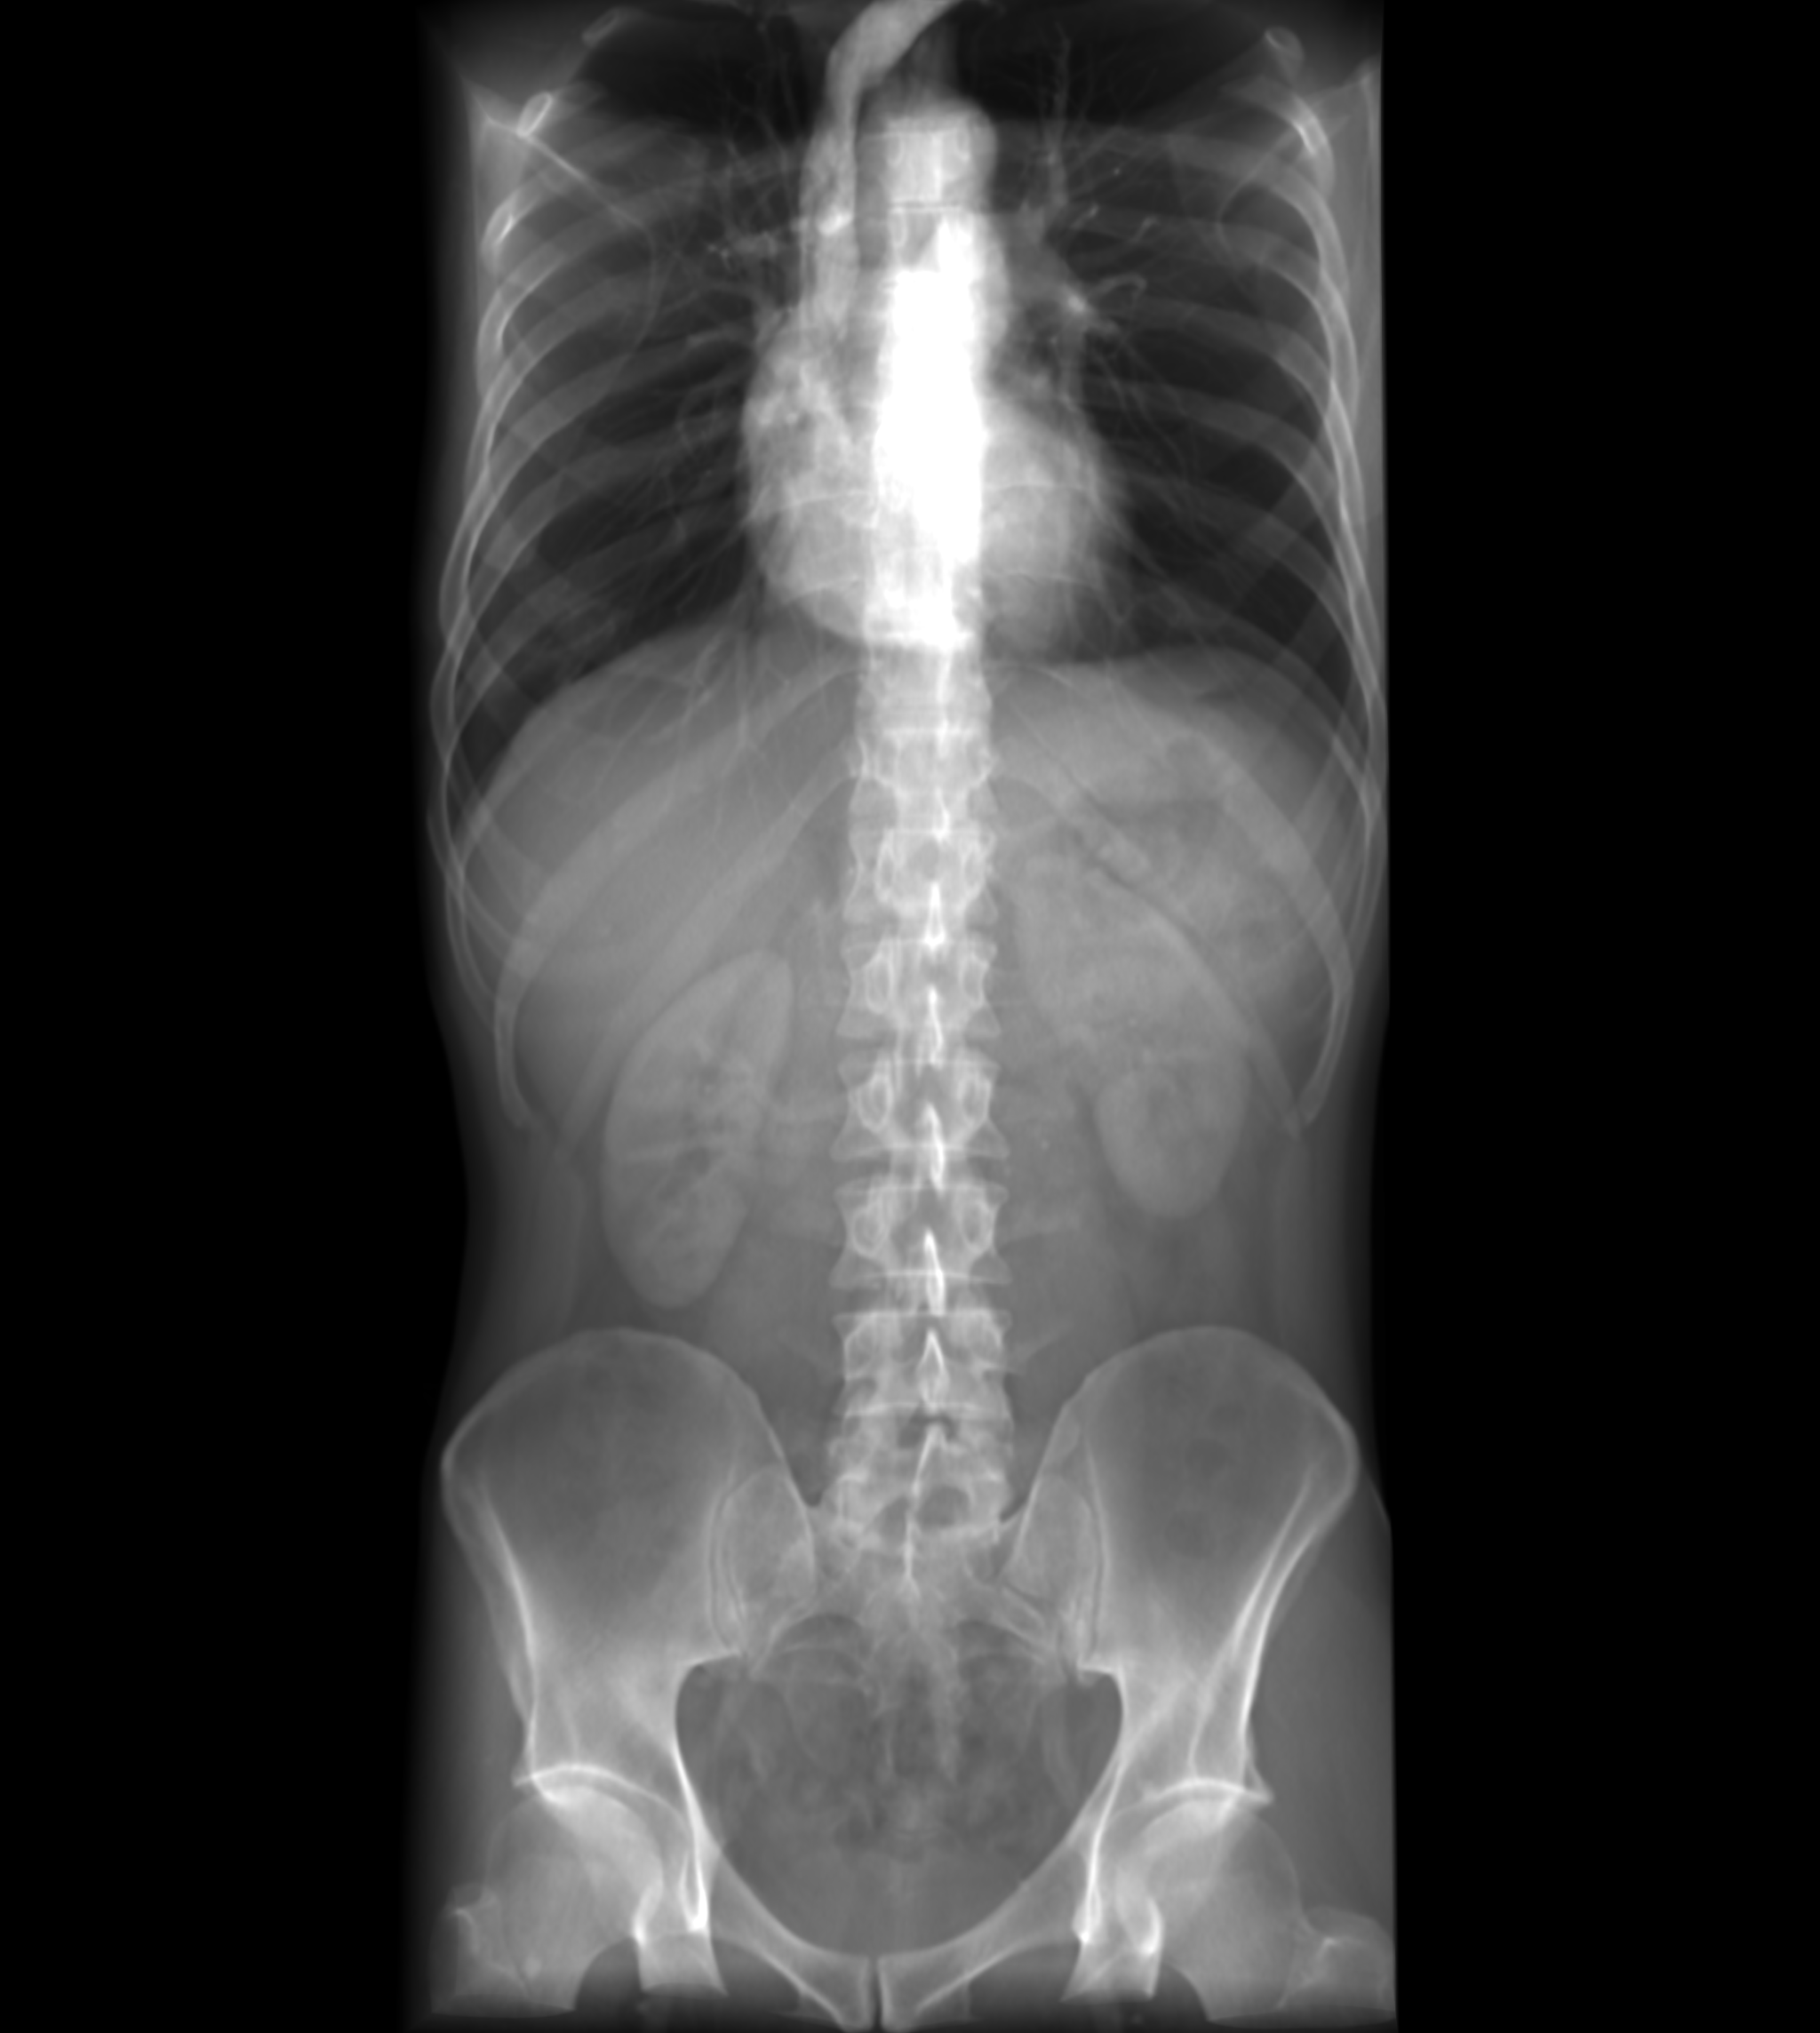
\includegraphics[width=\columnwidth]{TorsoBlendingAdditive.png}
\end{subfigure} 
\begin{subfigure}{.6\columnwidth}
    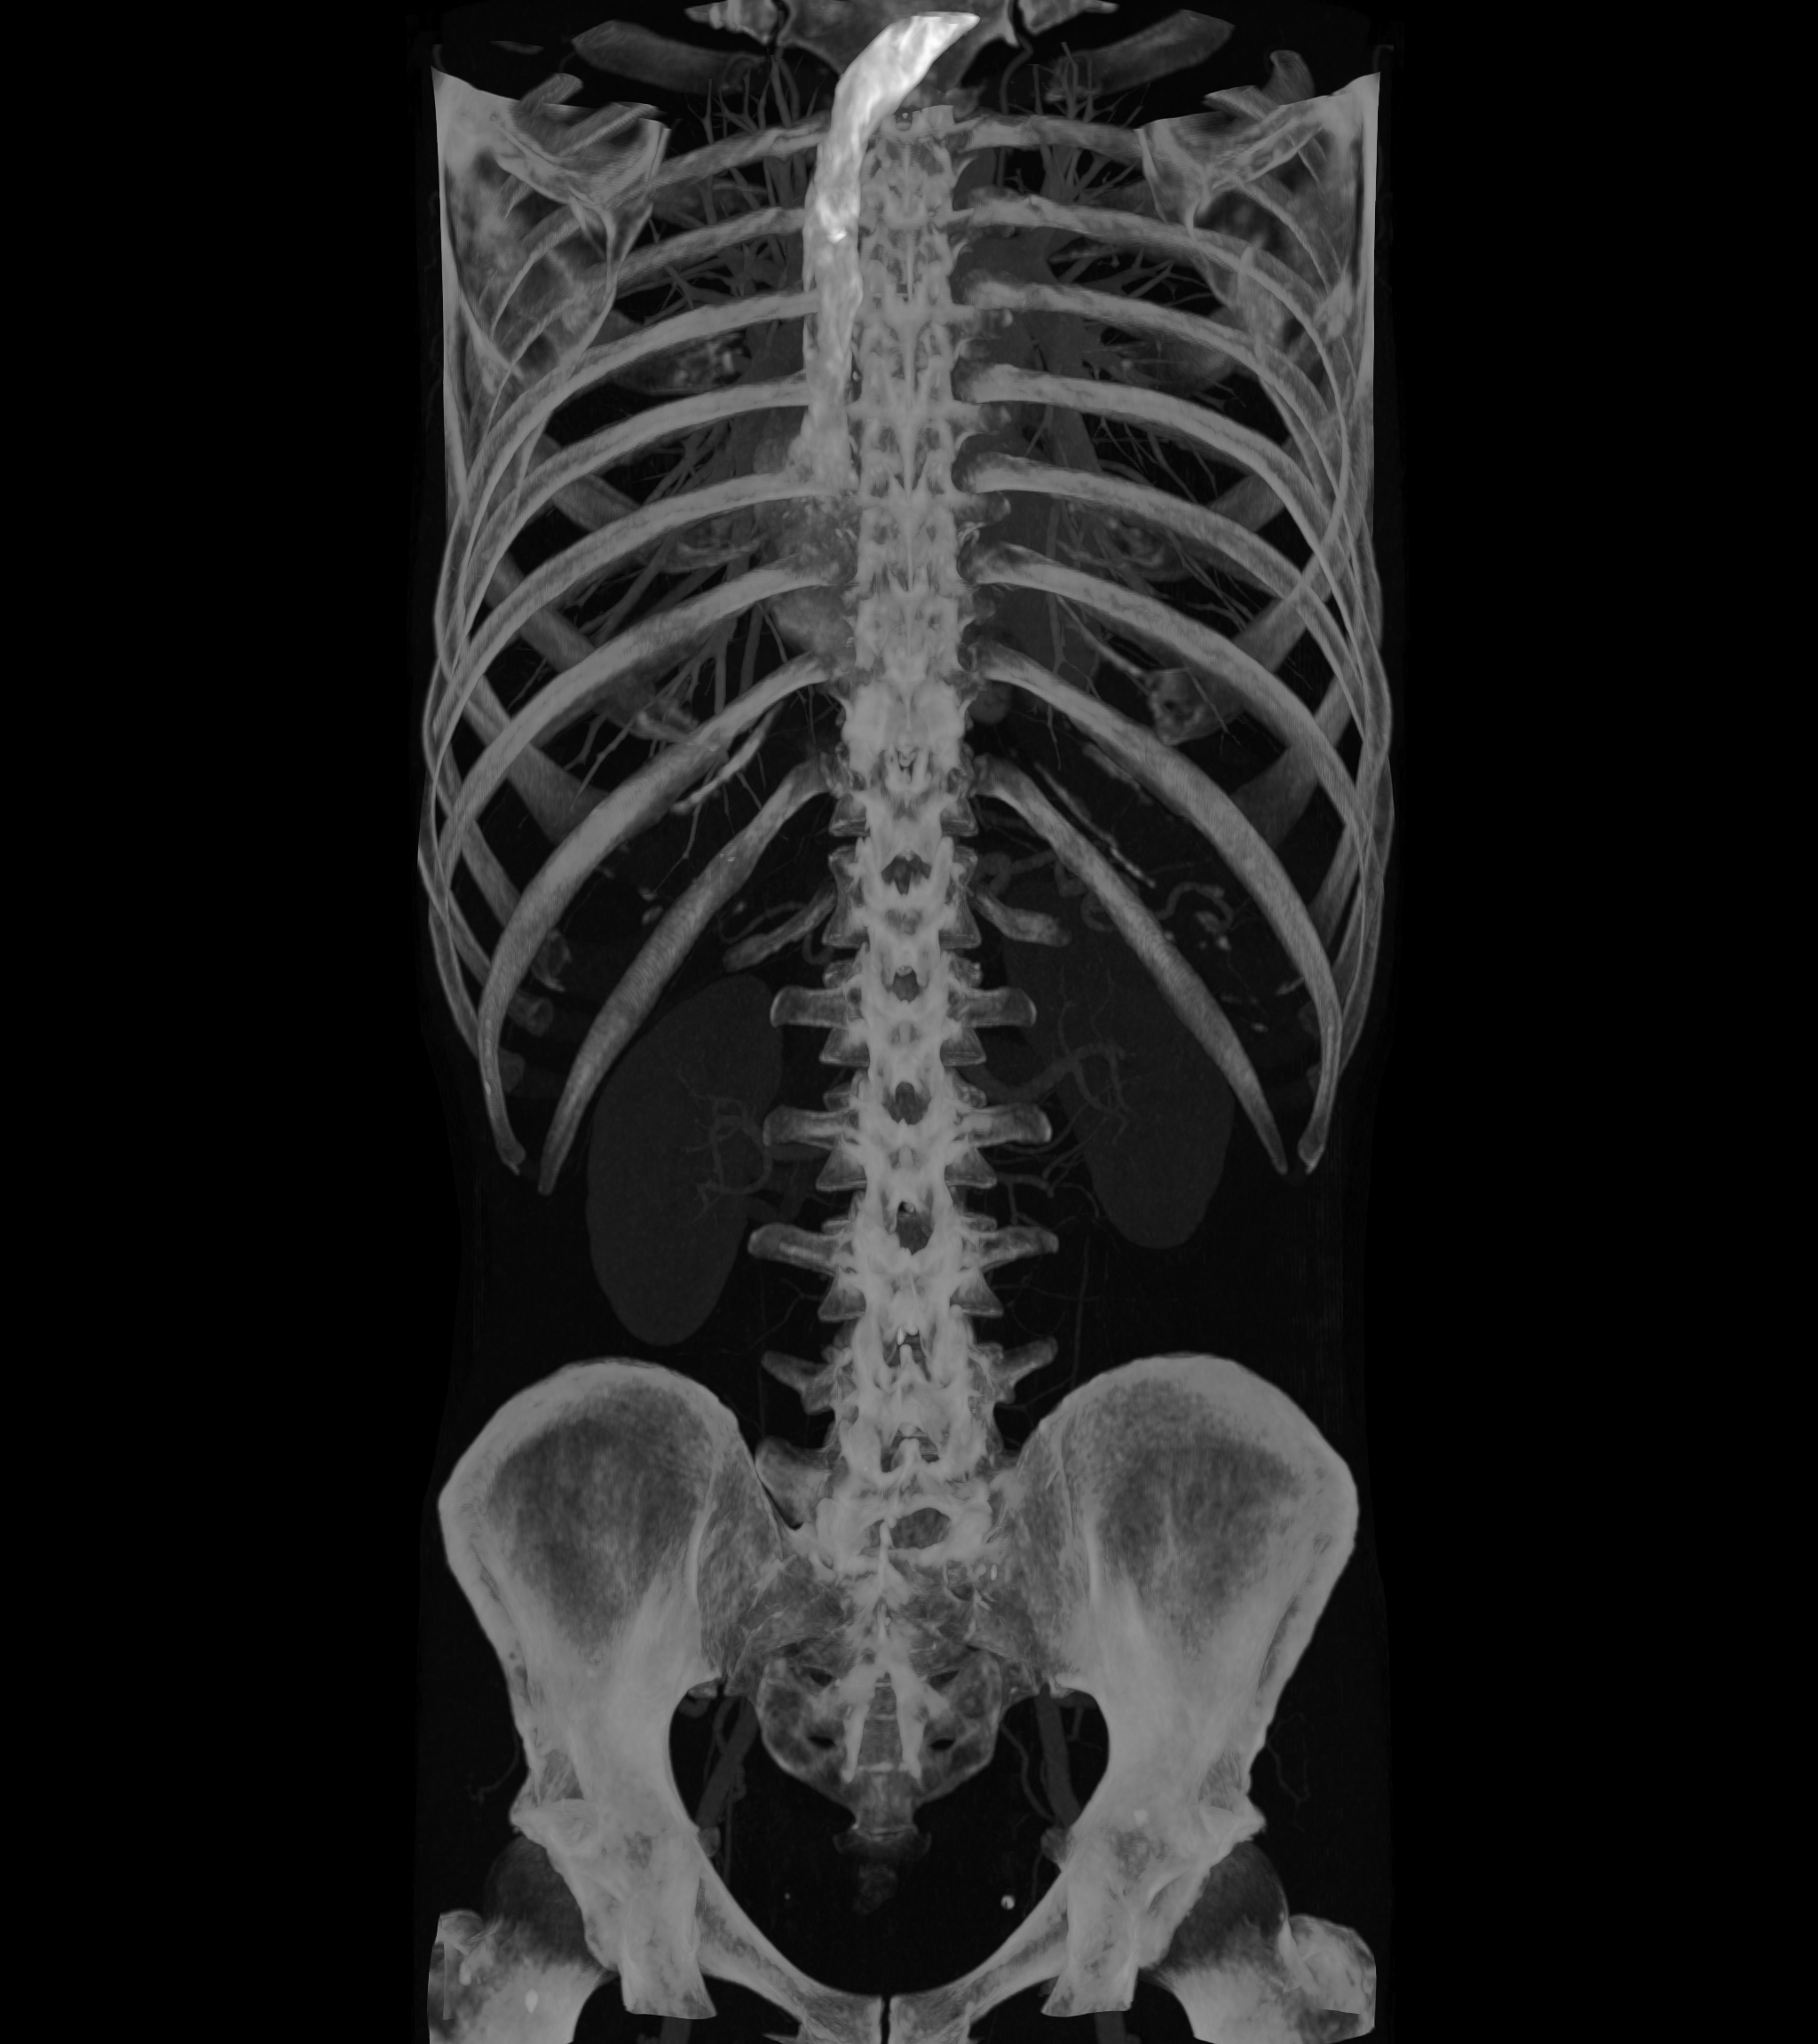
\includegraphics[width=\columnwidth]{TorsoBlendingMIP.png}
\end{subfigure}
\caption{Rendering with and without gradient opacity transfer function.}
\label{fig:blendingmodes}
\end{figure*}

\subsubsection{Masking}
Both binary and label masks are supported. With binary masks, the value in the masking volume indicates visibility of the voxel in the data volume. When a label map is in use, the value in the label map is used to select different rendering parameters for that sample.  See Figure 5 for an example of label data masks.

\subsubsection{Opacity Modulated by Gradient Magnitude}
A transfer function mapping the magnitude of the gradient to an opacity modulation value can be used to essentially perform edge detection (de-emphasize homogenous regions) during rendering. See ~\ref{fig:gradient} for an example of rendering with and without the use of a gradient opacity transfer function.

\begin{figure*}
\centering
   \begin{subfigure}[b]{0.5\textwidth}
   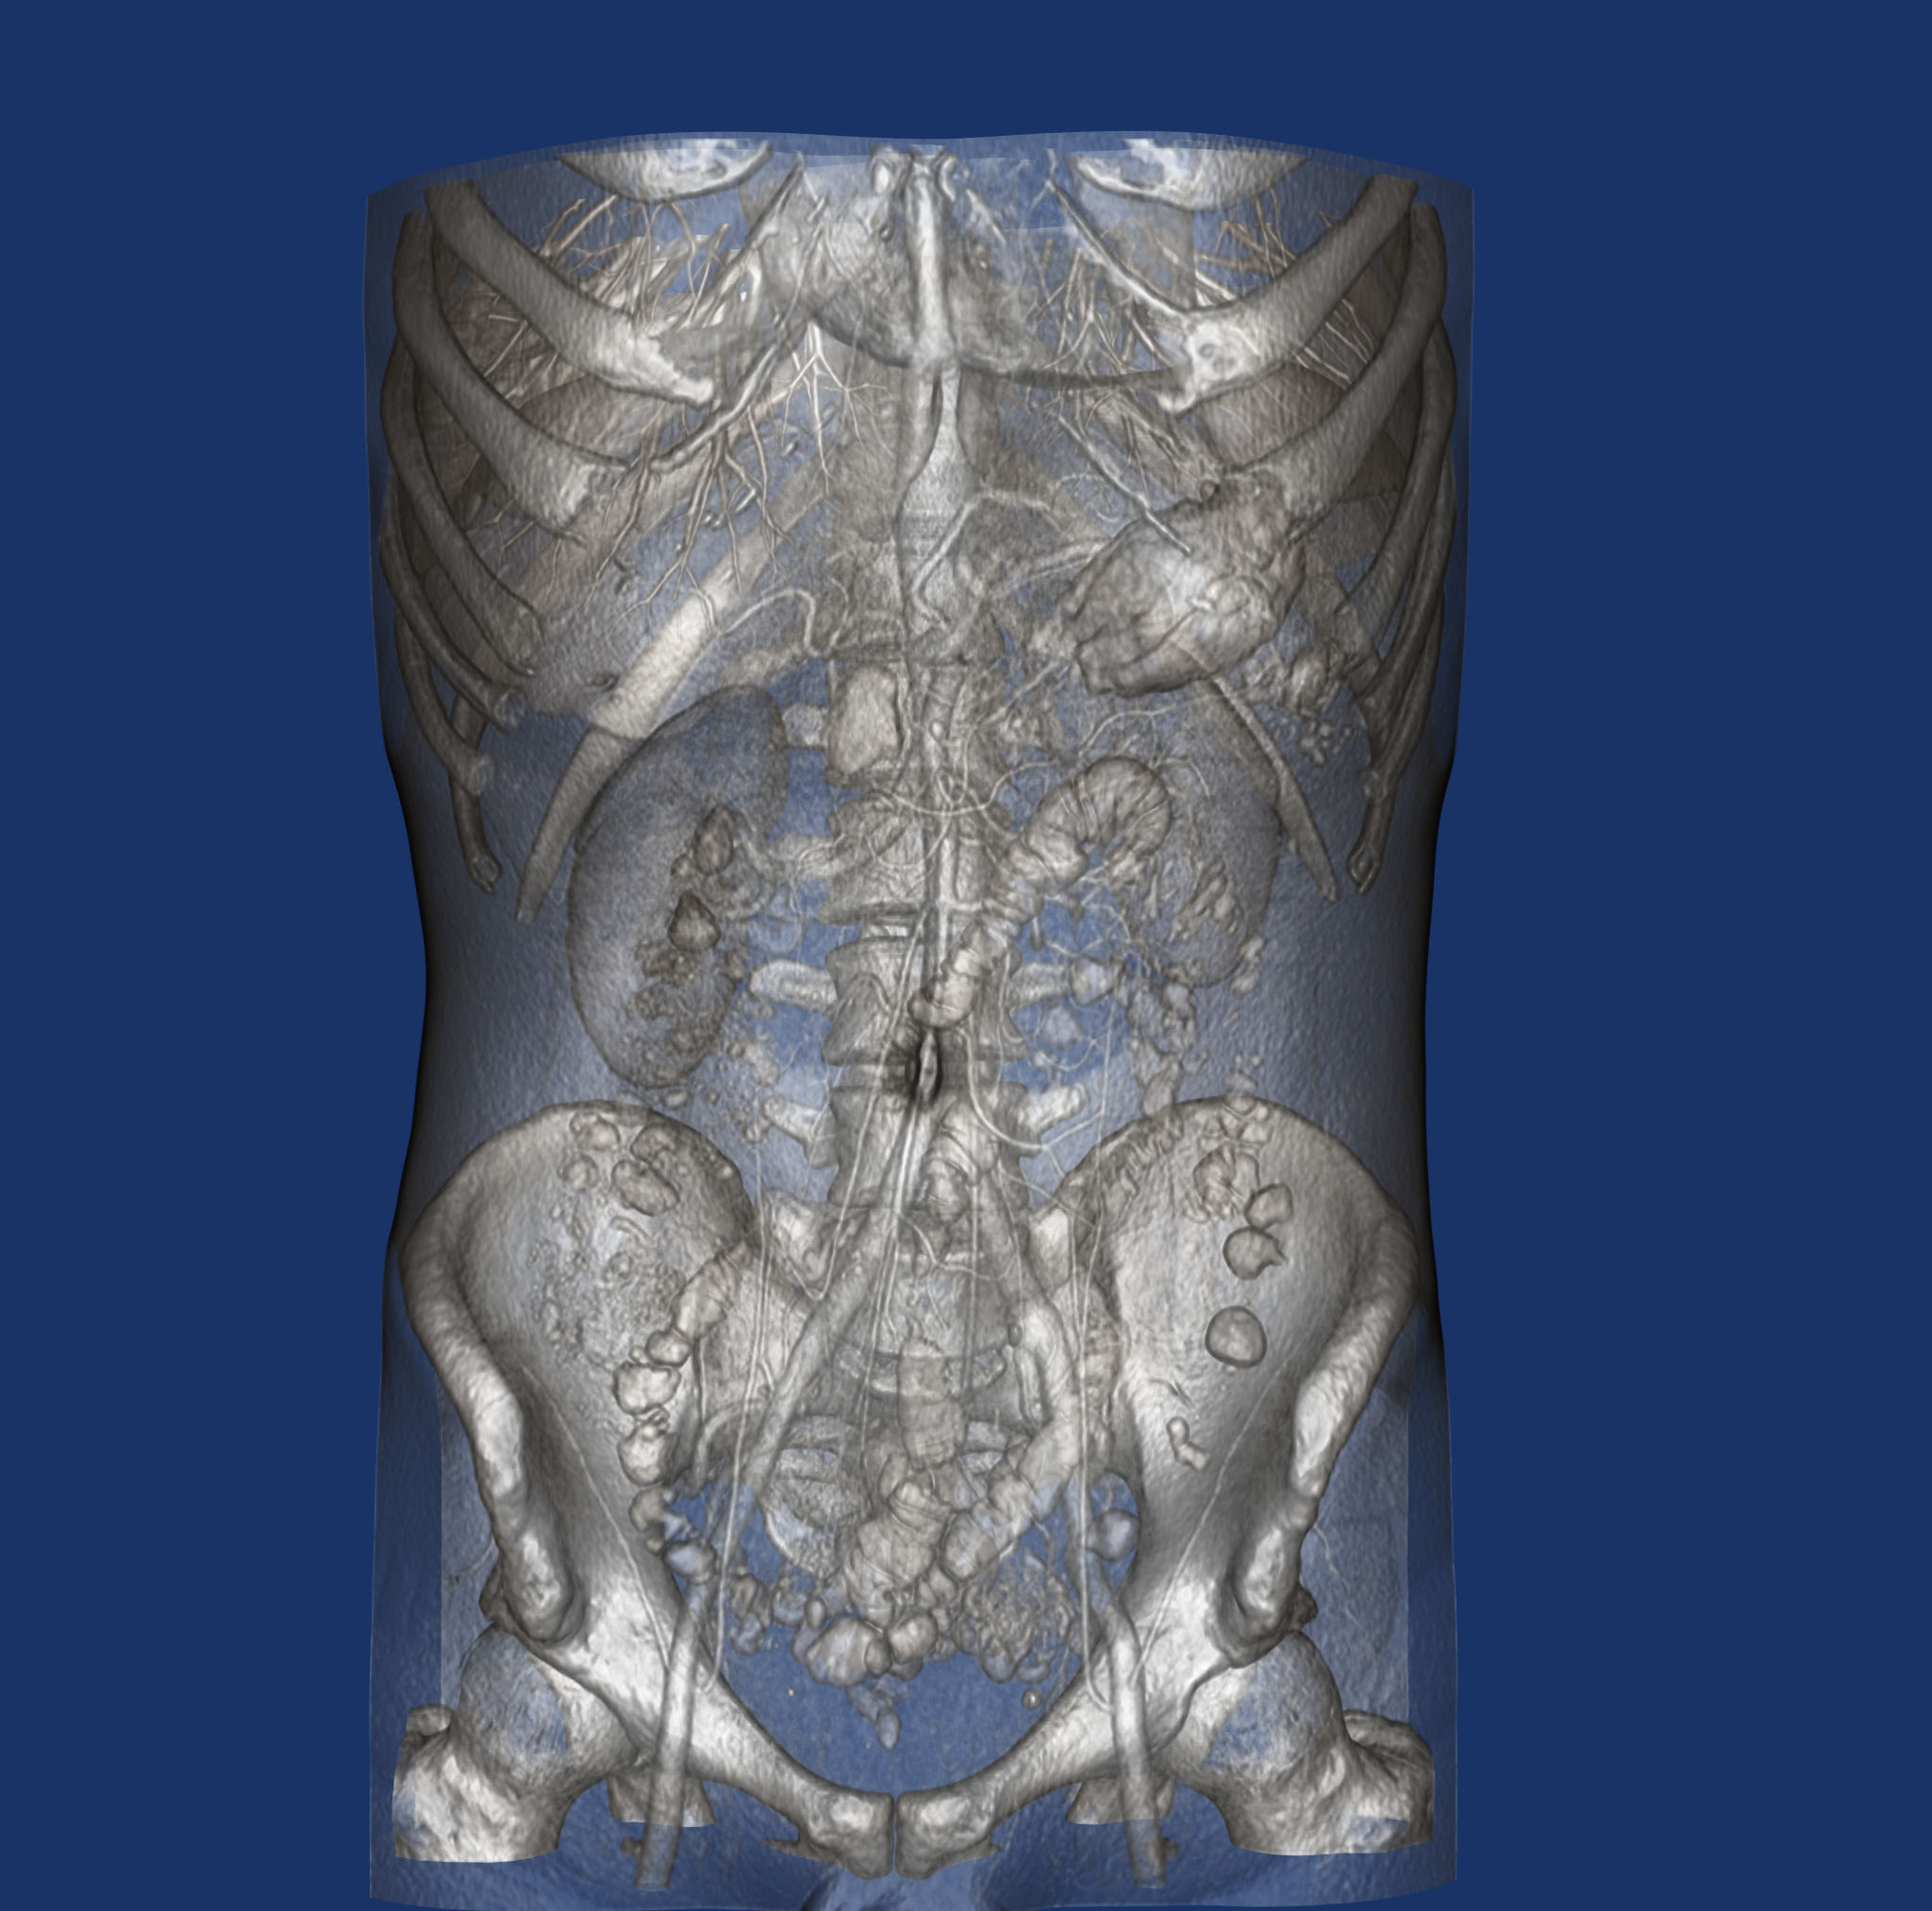
\includegraphics[width=1\linewidth]{TorsoGradient.png}
   \caption{}
   \label{fig:Ng1} 
\end{subfigure}

\begin{subfigure}[b]{0.5\textwidth}
   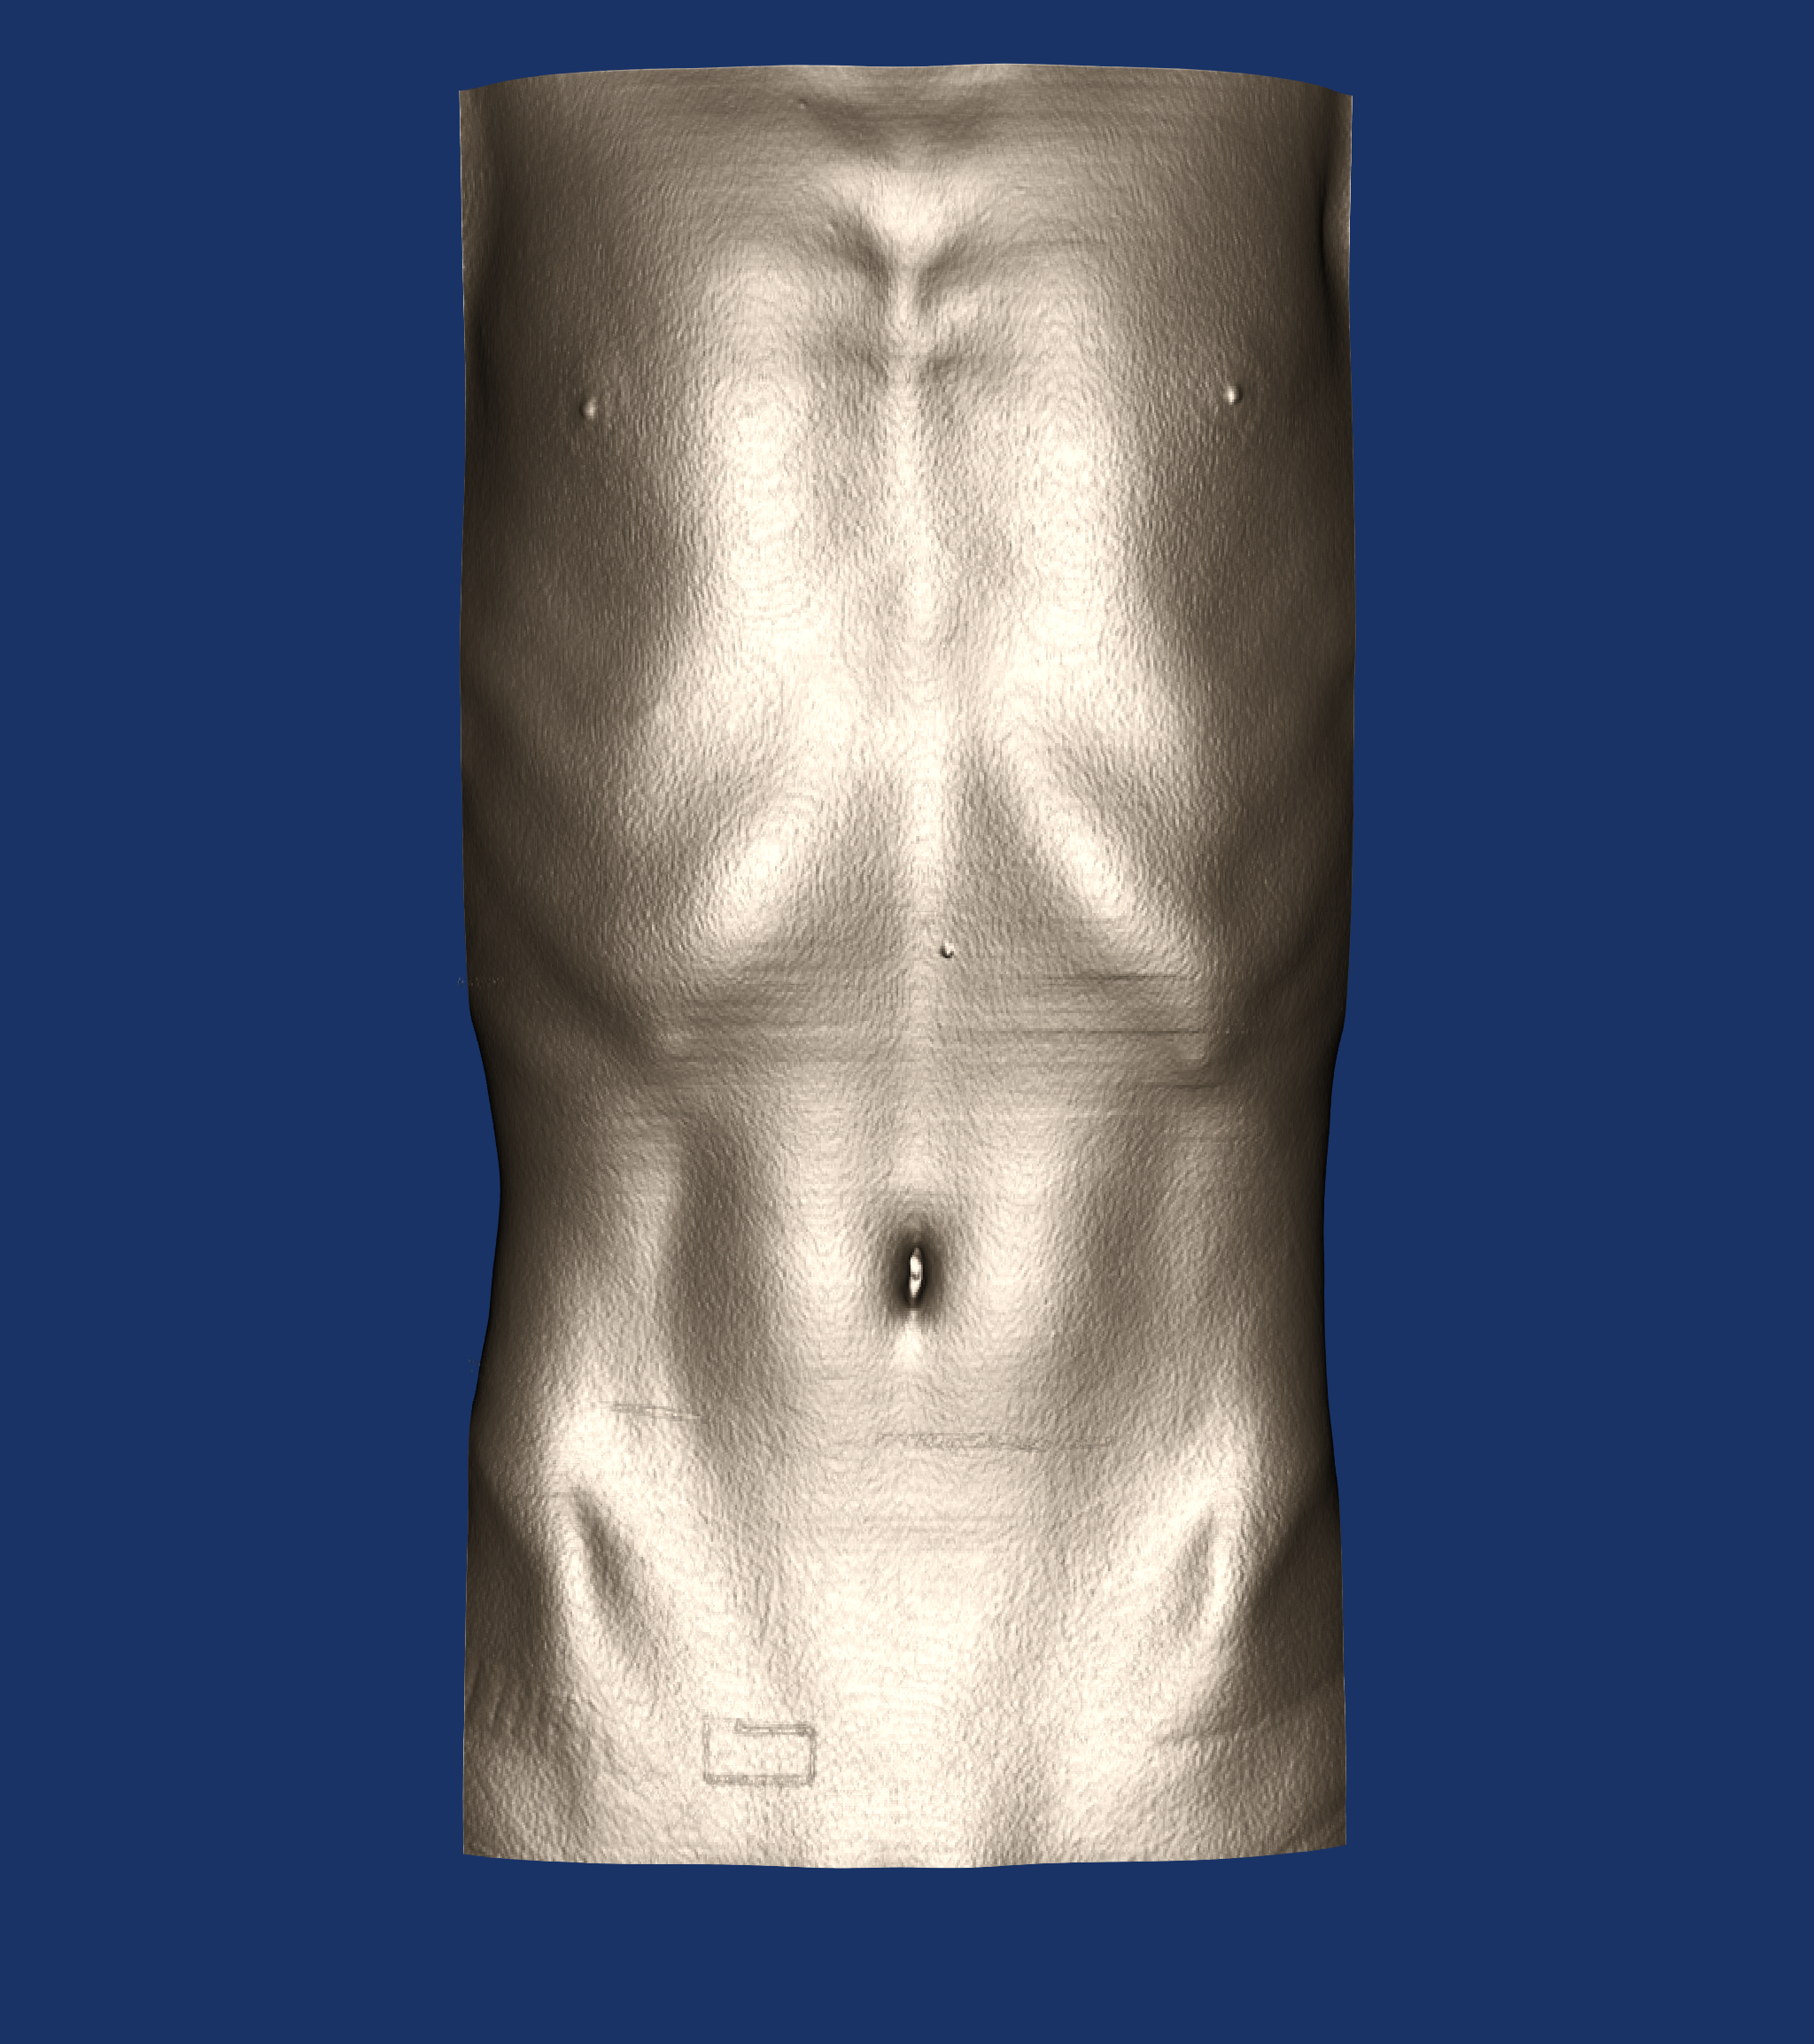
\includegraphics[width=1\linewidth]{TorsoNoGradient.png}
   \caption{}
   \label{fig:Ng2}
\end{subfigure}

\caption{Rendering with and without gradient opacity transfer function.}
\label{fig:gradient}
\end{figure*}